
\clearpage
\section{Importieren}
\label{bkm:Ref2018090701}

\begin{wrapfigure}[3]{l}{6.5cm}   % [x] Wie manche Zeile soll sich um die Grafik "brechen"
  \vspace{-35pt}      % Grundwert war 20; mit 30 schön oben beim Text ausgerichtet
  \begin{center}
    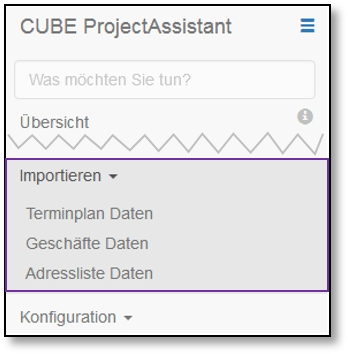
\includegraphics[width=1\linewidth]{../chapters/12_Importieren/pictures/12_Menu_Importieren.jpg}
  \end{center}
  \vspace{-20pt}
  \caption{Daten importieren}
  \vspace{-10pt}
\end{wrapfigure}

Wählen Sie im Menü links den Punkt 'Importieren' und dann den gewünschten Unterpunkt 'Terminplan Daten' oder 'Geschäfte Daten'.

\vspace{6.5cm}

\subsection{Terminplan Daten}
\label{bkm:Ref445411998}

\begin{wrapfigure}[10]{r}{6cm}
\vspace{-15pt}
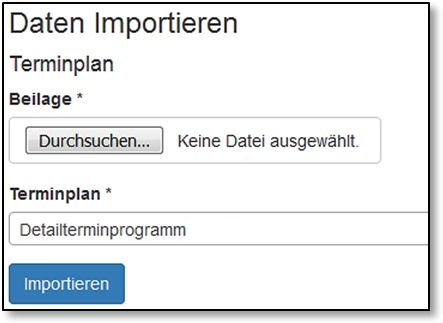
\includegraphics[height=50mm]{../chapters/12_Importieren/pictures/12-1_DatenImportieren.jpg}
\caption{Daten importieren}
\end{wrapfigure}
Mittels der Importier-Funktion 'Terminplan Daten' lässt sich ein neues, aktuelles Detailterminprogramm einlesen. Die Projektplanung erfolgt in Microsoft Project und wird als XML File exportiert und im CUBE PA importiert. Dabei gehen die bestehenden Daten im CUBE PA verloren. Die eingelesenen Daten können nicht geändert, sondern nur angezeigt werden. So ist es möglich auch auf Computern ohne Microsoft Project die Projektplanung einzusehen und nach gewünschten Zeitfenstern zu filtern. Weitere Informationen befinden sich im Kapitel \ref{bkm:Ref445400921} 'Die Terminplanung benutzen'.

\vspace{\baselineskip}

Um im CUBE PA die zusätzlichen Anzeige- und Filteroptionen (Projekt / Teilprojekt, Ressourcen) verwenden zu können, müssen die entsprechenden Informationen bereits im MS-Project File enthalten sein. Die Ressourcen werden dabei gemäss üblicher MS-Project Vorgehensweise vorgängig definiert und anschliessend den einzelnen Vorgängen zugewiesen. Die Zuordnung der Vorgänge zu einem Projekt / Teilprojekt wird mit Hilfe von benutzerdefinierten Feldern ermöglicht. Dazu sind im Project-File zwei neue Spalten hinzuzufügen (Typ Text, z.B. Text1 und Text2). Diese Spalten sind in der Gantt-Diagramm Ansicht entweder direkt in der Tabelle oder unter Format - Benutzerdefinierte Felder mit 'Subproject\_1' und 'Subproject\_2' zu benennen \col{(1)}. Dies ermöglicht das korrekte Einlesen der Daten im CUBE PA. Den einzelnen Vorgängen können anschliessend die Projekte (Teilprojekte) gemäss den Tag Definitionen in CUBE PA zugewiesen werden. Dies geschieht durch manuelle resp. Dropdown-Eingabe der Projektnamen in den Spalten 'Subproject\_1' und 'Subproject\_2'. Vor dem Export / Import sollte unbedingt geprüft werden, dass sämtliche Vorgänge den korrekten Projekten zugeordnet sind und keine Felder leergelassen wurden. Nur so kann verhindert werden, dass bei späterer Filterung in CUBE PA keine Vorgänge irrtümlicherweise ausgeblendet werden.

\begin{figure}[H]
\center{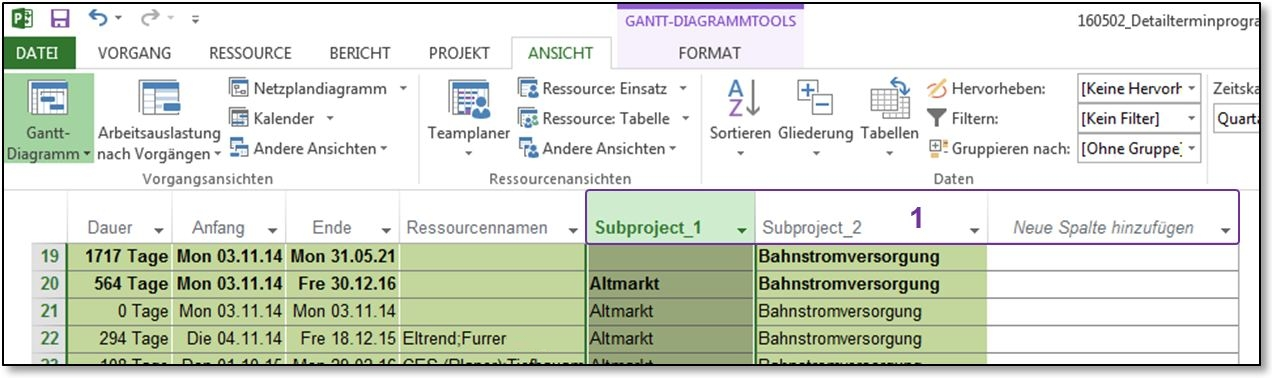
\includegraphics[width=1\linewidth]{../chapters/12_Importieren/pictures/12-1_zusSpaltenMSProject.jpg}}
\caption{Zusätzlich benötigte Spalten in MS-Project}
% \label{fig:speciation}
\end{figure}

\subsection{Geschäfte Daten}

Folgt später.

\subsection{Adressliste Daten}

Es ist möglich eine Adressliste, welche in Excel erstellt wurde oder im Excel-Format vorliegt, in den CUBE PA zu importieren. 

\begin{figure}[H]
\center{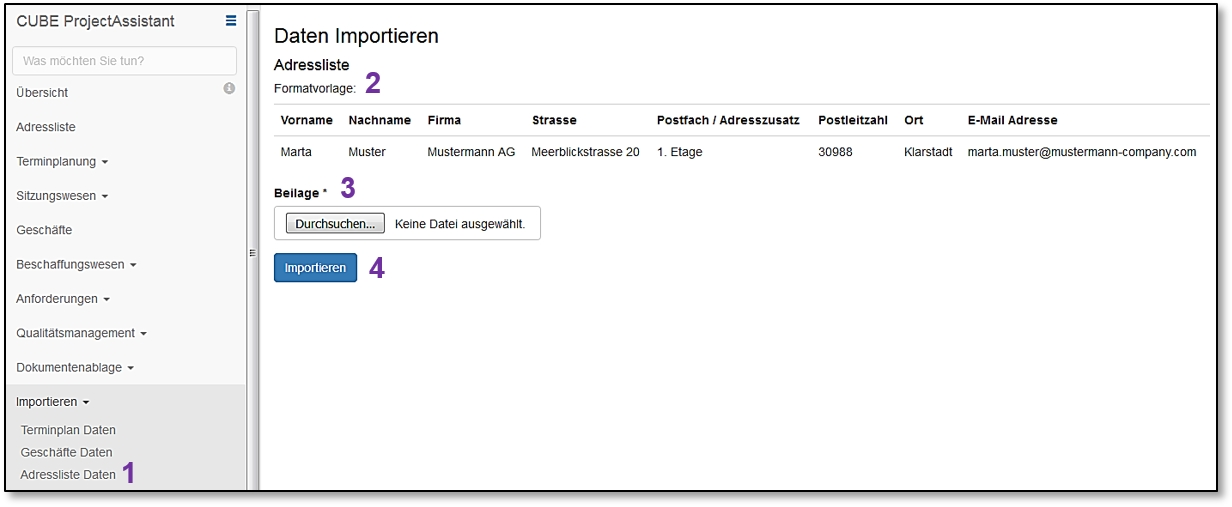
\includegraphics[width=1\linewidth]{../chapters/12_Importieren/pictures/12_Adressdaten_impUebersicht.jpg}}
\caption{Excel-Adressliste importieren}
% \label{fig:speciation}
\end{figure}

Klicken Sie im Menü links unter 'Importieren' auf den Menüpunkt 'Adressliste Daten' \col{(1)}. Sie sehen rechts unter 'Formatvorlage' \col{(2)}, welche Felder unterstützt werden und wie die Tabelle vorbereitet werden muss, damit der Import erfolgreich durchgeführt werden kann.

\vspace{\baselineskip}

Klicken Sie auf 'Durchsuchen' \col{(3)} und wählen Sie anschliessend die gewünschte Datei aus. Nach der Auswahl der Excelliste und Klick auf 'OK' können Sie überprüfen, welche Datei nun importiert werden soll:

\begin{figure}[H]
\center{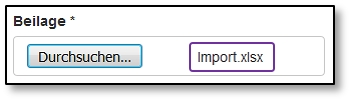
\includegraphics[width=.5\linewidth]{../chapters/12_Importieren/pictures/12_Listenimport.jpg}}
\caption{Datei auswählen}
% \label{fig:speciation}
\end{figure}

Ist alles korrekt, klicken Sie auf den Button 'Importieren' \col{(4)}, die Adressen werden importiert und sind anschliessend im Menü 'Adressliste' verfügbar. 

\vspace{\baselineskip}

Im Anschluss an den Import-Vorgang sehen Sie eine Auflistung der Adressen, welche hinzugefügt wurden und es ist ebenso ersichtlich, ob alles einwandfrei importiert wurde:

\begin{figure}[H]
\center{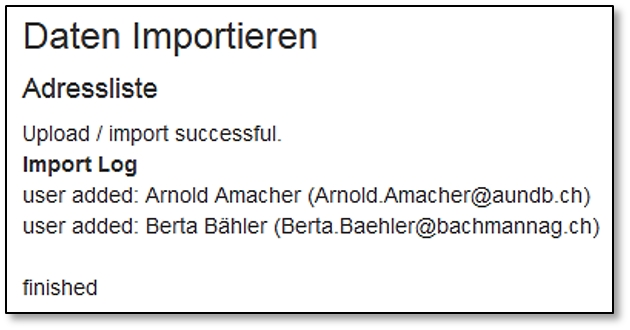
\includegraphics[width=.5\linewidth]{../chapters/12_Importieren/pictures/12_Import_ok.jpg}}
\caption{Import-Protokoll}
% \label{fig:speciation}
\end{figure}

Hätte etwas nicht funktioniert, sehen Sie an dieser Stelle eine Fehlermeldung.